\documentclass[a4paper,5pt]{thesis.cs.pub.ro}

\usepackage{graphicx}
\usepackage{subcaption}
\usepackage{ucs}
\usepackage[utf8x]{inputenc}
\usepackage{tikz}
\usetikzlibrary{shapes,arrows}
\usepackage{mathtools}

\makeatletter
    \setlength\@fptop{0\p@}
\makeatother

\begin{document}

\titleen{A Scalable Algorithm for Similar Image Detection}
\author{Andrei-Bogdan P\unichar{226}rvu}
\date{iulie 2014}
\adviser{\\Prof. Dr. Ing. Nicolae \unichar{538}\unichar{259}pu\c{s}\\Ing. \c{S}tefan-Teodor Cr\unichar{259}ciun}

\begin{titlepage}
\begin{center}
{\Large University ``POLITEHNICA'' of Bucharest}
\par\vspace*{2mm}
{\Large Automatic Control and Computers Faculty,

  Computer Science and Engineering Department}
  \par\vspace*{3mm}
  \begin{table*}[h]
  \begin{center}
  \begin{tabular}{cccc}
  
\includegraphics[width=0.13\textwidth]{images/brand/upb}
  & & &
  
\includegraphics[width=0.30\textwidth]{images/brand/cs}
  \end{tabular}
  \end{center}
  \end{table*}

  \par\vspace*{25mm}
{\Huge BACHELOR THESIS}
\par\vspace*{15mm}
{\Huge \VARtitleen }
\par\vspace*{35mm}
\begin{table*}[h]
\begin{center}
\begin{tabular}{lcccccl}
\Large \textbf{\Large Scientific Advisers:}
\vspace*{1mm} &&&&&& \Large \textbf{\Large Author:}\vspace*{1mm} \\
    \Large \VARadviser &&&&&& \Large \VARauthor
    \end{tabular}
    \end{center}
    \end{table*}

    \par\vspace*{30mm}
    \Large \VARtitlefooteren
    \end{center}
    \end{titlepage}



\tableofcontents

\begin{abstract}
In this paper, I propose an algorithm for detecting similar images in a large scale dataset, with the goal of obtaining a method of determining the appearance of copyright infringement. After considering various methods as invisible watermarking and image feature detection, I decided upon using the $Harris\ corner\ detection$ and the $Scale\ Invariant\ Feature\ Transform$ keypoints and descriptors for analyzing the properties of an image.\\
In order to be able to handle a large amount of images and associated data, I have decided to maintain the descriptors of the images in a KD-tree structure for fast querying. This allows an initial filtering of the data set, reducing the number of images which should be analyzed. Thus, I will use two algorithms, one of which has a lower time complexity, but only gives semi-accurate results, and a second one, which performed a more in-depth analysis of the images.\\
I will describe the mathematical aspects of the two mentioned algorithms, and I will describe the adjustments made to the algorithms in order to perform better on our given problem.\\
The architecture of the application also important, because it highly influences the distribution of data, and how the algorithm performs on a large data set, with a high number of queries and possible updates on the initial image set. I will describe this architecture and the way the data should be distributed so that an efficient use of multiple machines can speed up the algorithm.\\

\end{abstract}

\chapter{Introduction}

Image processing has been a very important research domain the last years, the ever increasing number of images present on the Internet becoming more and more challenging to index, store and analyze.\\
Privacy and copyright have also been big issues which have been discussed and assessed for a long time, major users in the photography industry wanting to know at all times when someone is using or modifying one of their photos.

\section{Requirements}

We want to design a scalable algorithm which can maintain a large set of images, and perform queries of finding a highly similar image with a given input one. \\
The algorithm should be focused on copyright detection, so it should be able to determine if the input image is one of the images in the dataset, with possible transformations applied upon it:
\begin{itemize}
	\item watermarks
	\item scaling
	\item cropping
	\item various filters
\end{itemize}

As said above, the granularity of the algorithm should be able to distinguish between two lightly similar images (e.g. two different pictures of the Eiffel Tower, made by two different persons) and two images, one of which is obtained from the other.\\

The running time of the algorithm is also a major factor which should be seriously taken into consideration. It should be able to handle a large number of queries and provide a small response-time per query. Of course, there is a close connection between the running time of the algorithm and its precision, connection which should be closely analyzed in order to create a balance between the two.

In Figure~\ref{fig:basicUsage}, we can see an example usage of the algorithm. The large database is queried with the image in the bottom-left corner, and the algorithm is capable is returning the original image (even if the query image has been cropped, rotated and a gray filtered applied).

\begin{figure}[ht!]
\centering
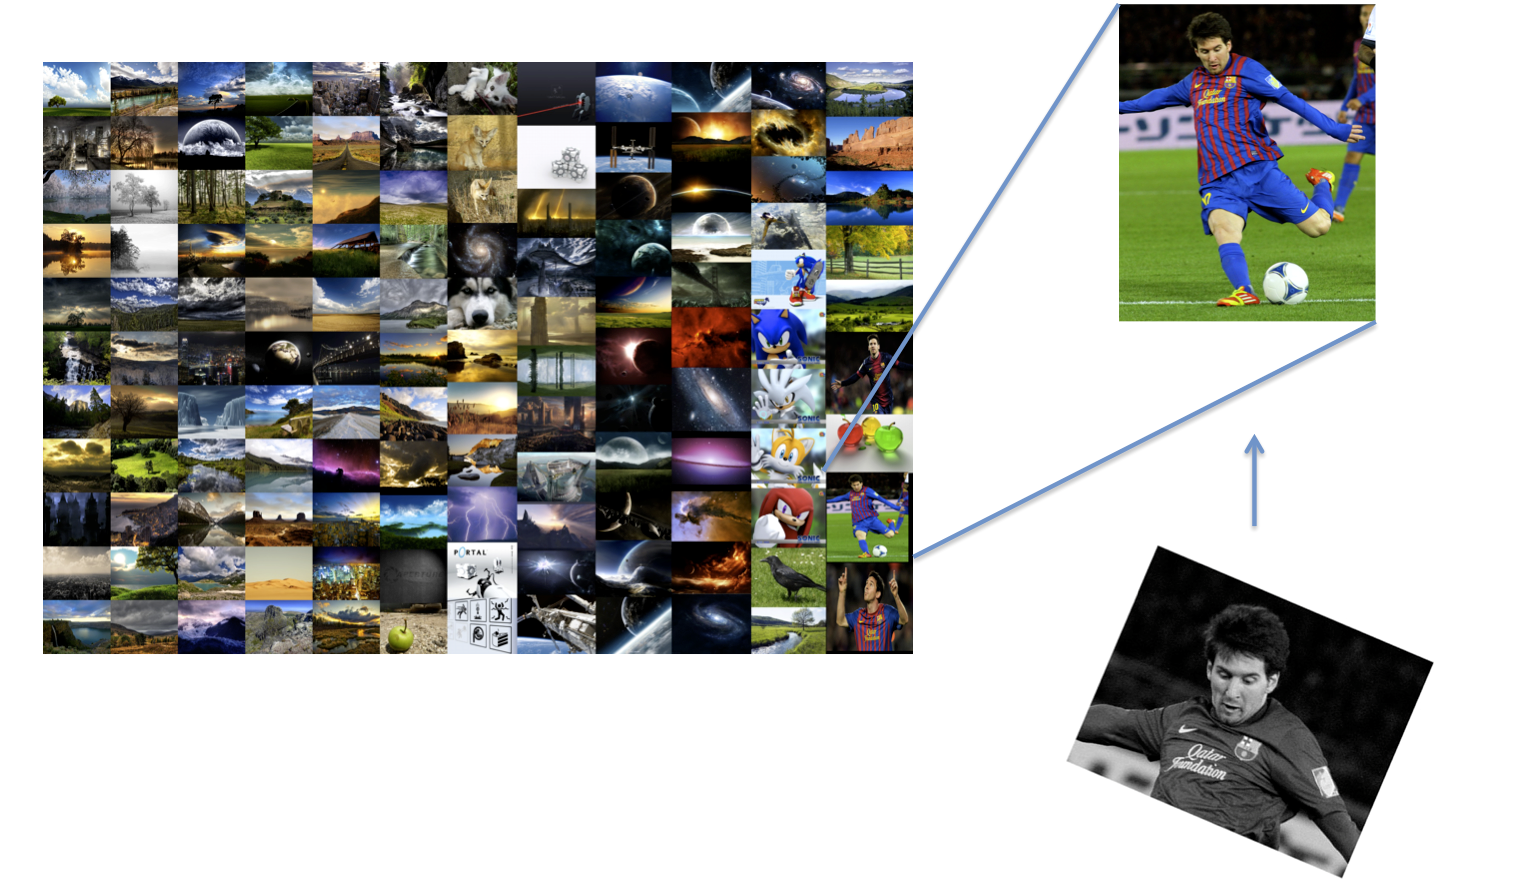
\includegraphics[width=.8\linewidth]{images/basicUsage.png}
\caption{Basic usage of our algorithm}
\label{fig:basicUsage}
\end{figure}

\chapter{Related Work}
\label{chap:relatedWork}

There are a lot of algorithms which focus on image similarity and key feature detection, our main goal being to select specific ones on which we can control the sensitivity of the matches, but also which can be easily and efficiently distributed on several machines for a large input set. \\
We have focused on two main algorithms, the $Harris\ corner\ detector$ and the $Scale\ Invariant$ $Feature\ Transform$.


\section{Harris Corner Detection}

The main idea of the $Harris\ corner\ detector$ \cite{harrisCorner}, \cite{harrisCorner2} algorithm is that, given an input image, the most predominant features that a human eye recognizes and memorizes are corners. A corner is considered to be an intersection of two edges, so, selecting a small area around the point and shifting it should result in a large variation in the intensity of the pixels in that area. \\
Therefore, each area in an image can be classified in three categories:
\begin{itemize}
	\item flat, in which intensities do not vary in either direction (as seen in Figure~\ref{fig:flatArea})
	\item edge, in which intensities don't vary in the direction of the edge (as seen in Figure~\ref{fig:edgeArea})
	\item corner, in which intensities vary in all directions (as seen in Figure~\ref{fig:cornerArea})
\end{itemize}

In order to determine in which category a certain area with a size of $(w, h)$ belongs to, we will compute the variation of intensity: $E(w, h) = \sum_{x, y} w(x, y) * [I(x + w, y + h) - I(x, y)]^2$, where $w$ is a window function, which assigns weights to pixels, and $I$ is the intensity of a certain pixel of the grayscale image.\\
In order to determine the corner areas, we have to maximize the function $\sum_{x, y}[I(x + w, y + v) - I(x, y)]^2$, which, using $Taylor$ expansion and representing in a matrix form, can be written as
$E(w, h) \approx
\begin{bmatrix}
w & h
\end{bmatrix} * 
\left(\sum_{x, y}
\begin{bmatrix}
I_x^2 & I_xI_y\\
I_xI_y & I_y^2
\end{bmatrix}
\right) *
\begin{bmatrix}
w \\
h
\end{bmatrix}$, and, furthermore, using a substitution
$E(w, h) \approx
\begin{bmatrix}
w & h
\end{bmatrix} * 
M *
\begin{bmatrix}
w \\
h
\end{bmatrix}$.\\
Using this equation, the score of a certain area is computed as $R = det(M) - k * (trace(M))^2$. A higher score of $R$ denotes a higher probability of the area being a corner.

\begin{figure}[ht!]
\centering
\begin{minipage}{.5\textwidth}
	\centering
	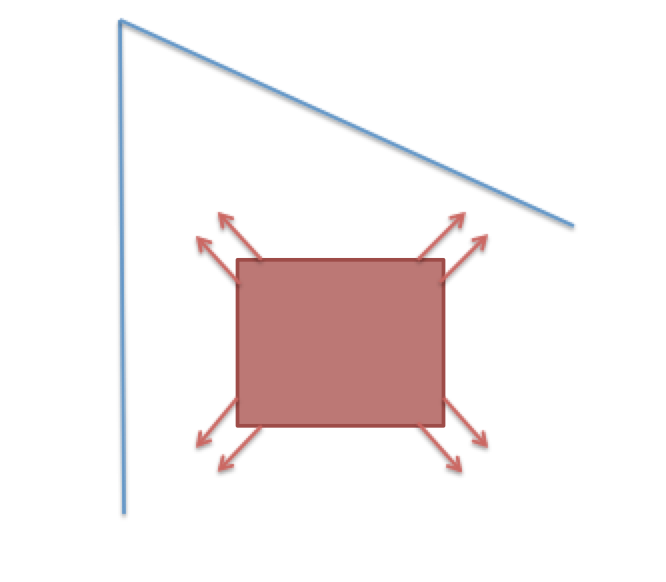
\includegraphics[width=.6\linewidth]{images/flatArea.png}
	\caption{Flat Area}
	\label{fig:flatArea}
\end{minipage}%
\begin{minipage}{.5\textwidth}
	\centering
	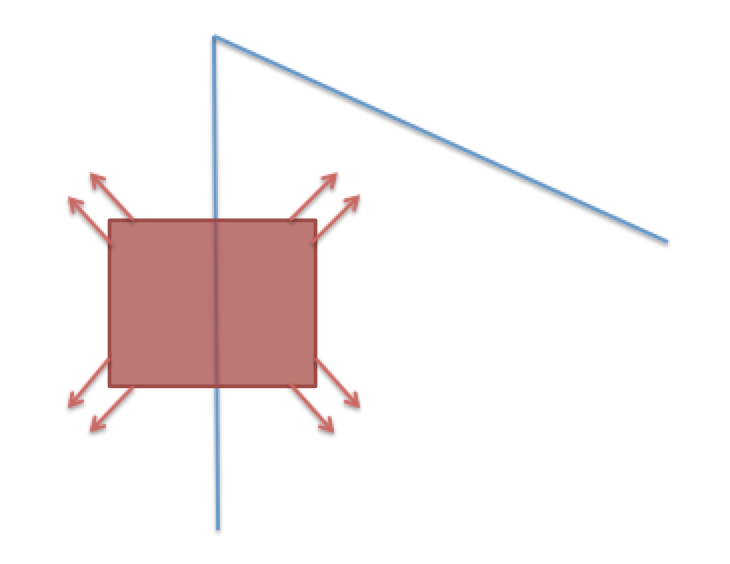
\includegraphics[width=.6\linewidth]{images/edgeArea.png}
	\caption{Edge Area}
	\label{fig:edgeArea}
\end{minipage}
\begin{minipage}{.5\textwidth}
	\centering
	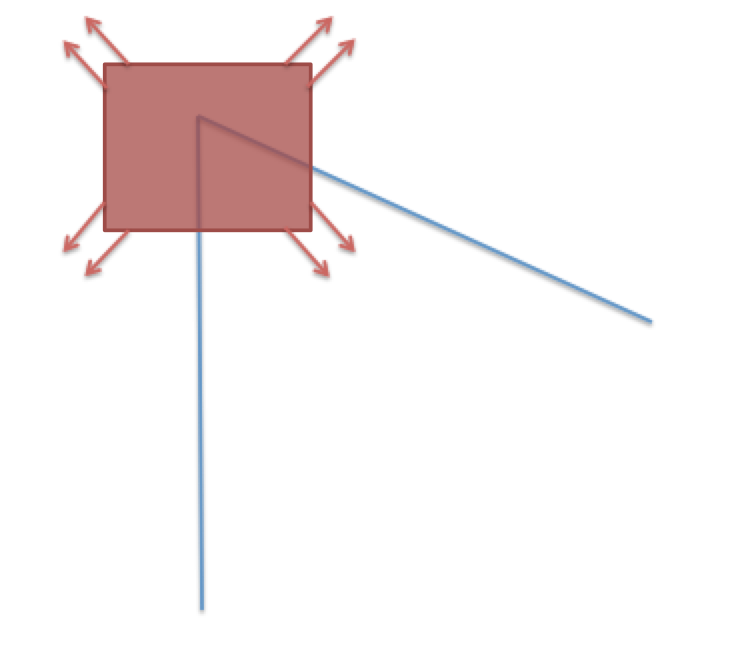
\includegraphics[width=.6\linewidth]{images/cornerArea.png}
	\caption{Corner Area}
	\label{fig:cornerArea}
\end{minipage}
\end{figure}


\section{Scale Invariant Feature Transform}
\subsection{Keypoint localization}
Although the $Harris\ corner\ detection$ algorithm presented in the previous section is immune to rotation transformations of an image, it does not perform well if the image is scaled, because a high intensity change in an area of size $(w, h)$ of an image might vary if the dimensions of the image change, but the size of the area remains the same.\\
Thus, David Lowe, in \cite{siftLowe}, presented a new algorithm for extracting keypoints and computing their descriptors, named $Scale\ Invariant\ Feature\ Transform$.\\
At first, a Gaussian distribution is applied on the analyzed image, which depending of the standard deviation, $\sigma$, blurs the image with a certain amount: $G(x, y) = \frac{1}{2 * \pi * \sigma^2} * e^{-\frac{x^2 + y^2}{2 * \sigma^2}}$.\\
Then, the Laplacian of the image is computed, in order to highlight the regions of rapid intensity changes: $L(x, y) = \frac{\delta^2 I}{\delta x^2} + \frac{\delta^2 I}{\delta y^2}$. Combined with the previous Gaussian filter, we obtain the so called Laplacian of Gaussian: $LoG(x, y) = -\frac{1}{\pi * \sigma^4} * \left(1 - \frac{x^2 + y^2}{2 * \sigma^2}\right) * e^{-\frac{x^2 + y^2}{2 * \sigma^2}}$.\\
Because the $LoG$ has a high computational cost, it is approximated with a Difference of Gaussians, which is a difference of two Gaussians with two different $\sigma$ deviations, representing two different scaled images. The local extrema of the computed $DoG$ are considered potential keypoints.

\subsection{Computing the Descriptors}
Once we have the keypoints, we have to compute a unique fingerprint for a given keypoint, which should be invariant to scaling, rotation and luminance \cite{siftImplementation}.\\
A $16\times16$ window is selected around a keypoint, which is divided into $16$ $4\times4$ blocks.
In each of these blocks, the gradient magnitude and orientation are computed for each of the $16$ elements.
These gradients are then inserted in an $8$ bin histogram. The histogram is computed using the following principles:
\begin{enumerate}
	\item the gradients are placed in the corresponding bin after their orientation: a gradient in range $0^o-44^o$ is placed in the first bin, a gradient in range $45^o-89^o$ is placed in the second, etc.
	\item the value added to the corresponding bin depends on the gradient magnitude
	\item also, the amount added to the corresponding bin depends on the distance from the keypoint. This is done using a gaussian weighting function
	\item to achieve rotation independence we have to subtract the keypoint's  orientation of the orientation of the histograms.
\end{enumerate}

After this computation, we remain with $16$ $8$ bin histograms, so we get a total of $128$ numbers.
The corresponding descriptors are computed by taking a $16\times16$ neighborhood around the keypoint, and creating a $8$ bin histogram for each sub-block of $4\times4$ size of the initial neighborhood. Thus, a keypoint descriptor will contain $128$ values.
These values are then normalized, and the descriptor of the current keypoint is obtained.

\begin{figure}[ht!]
\centering
\begin{minipage}{.5\textwidth}
	\centering
	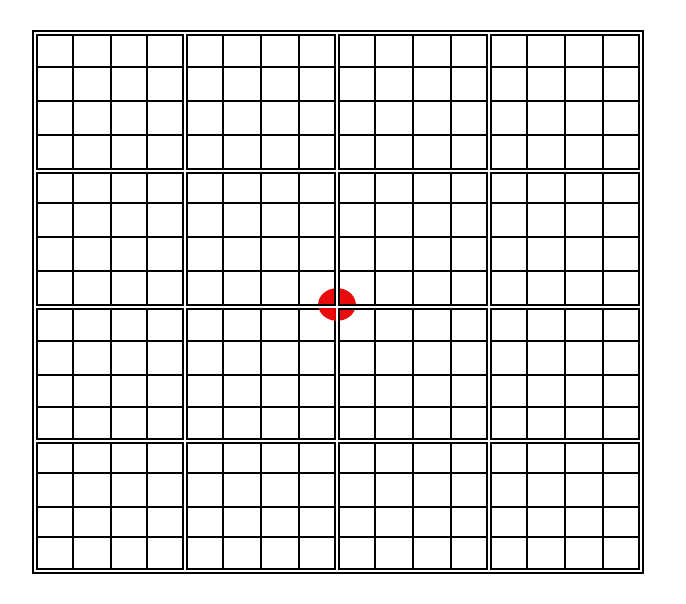
\includegraphics[width=.9\linewidth]{images/spacePartition.png}
	\caption{$16\times16$ window surrounding a\\ keypoint}
	\label{fig:spacePartition}
\end{minipage}%
\begin{minipage}{.5\textwidth}
	\centering
	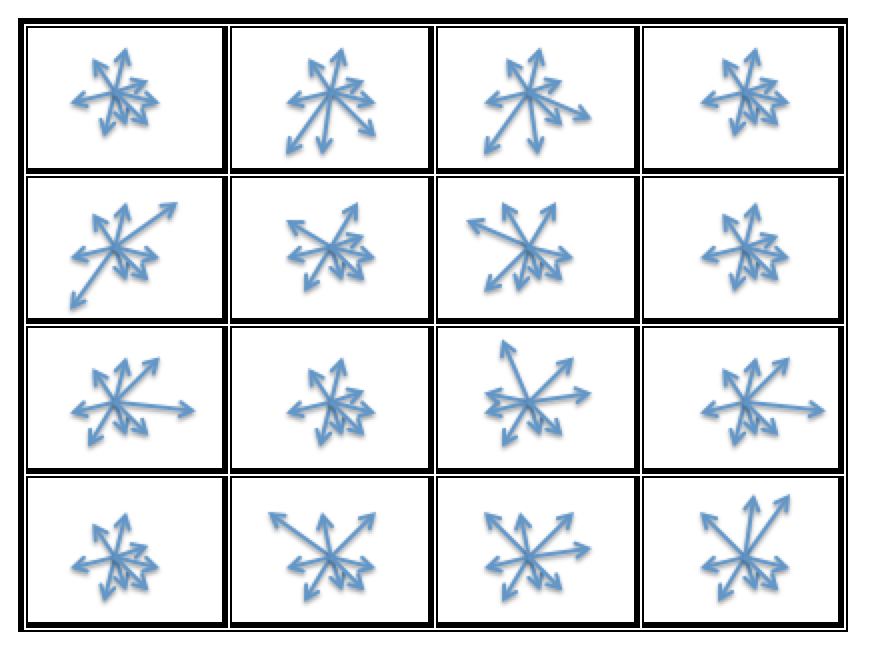
\includegraphics[width=1.1\linewidth]{images/imageGradients.png}
	\caption{Orientation histograms for the\\$4\times4$ window}
	\label{fig:imageGradients}
\end{minipage}
\end{figure}

\section{Speeded Up Robust Features}

SURF (Speeded Up Robust Features) is an algorithm which was introduced in 2006 as a speeded-up version of SIFT \cite{surf}. Insead of approximating the Laplacian of Gaussian with Difference of Gaussian, as SURF does, It approximates it with the Box Filter.\\
It uses wavelet responses \cite{haarWavelet}, \cite{haarWavelet2} on the X and Y axes to determine orientation assignment, which are plotted in a 2D space and summed up in a sliding window of $60^o$.\\
The wavelet responses are used again to compute the descriptors for the keypoints: a 4-dimensional vector $(\sum{d_x}, \sum{d_y}, \sum{|d_x|}, \sum{|d_y|})$ is computed for each block of size 4x4, thus obtaining a final descriptor of size 64.\\
We were interested in this descriptor, because of its similar performance with the SIFT descriptor, but lower dimension and faster computation.\\

\section{Descriptor Compression}

In \cite{descCompression}, a method is proposed for compressing SIFT and SURF descriptors, reducing their dimension and creating a metric which could be used to compute the distance between two compressed descriptors without requiring their decompression.\\
This method has four parts:
\begin{enumerate}
	\item a matrix which normalizes each row of a certain descriptor
	\item a distance lookup matrix 
	\item a weight vector, which assigns each row of a descriptor a certain weight depending on how much it will contribute to the final distance
	\item a tree coding scheme, similar to Huffman trees, which compresses the descriptors
\end{enumerate}

This is particular interesting for us because it can refuse the dimensionality of our problem, and provide a similar query response with a smaller running time.


\chapter{Design of the Algorithm}
\label{chap:design}

\section{Analysis of an image}

\subsection{Using Harris corner detector}
The analysis of an image begins with applying the Harris detector on it. It will compute a given score for each pixel of the image, the higher the score, the greater the chance that pixel represents a corner.\\
Using these values we will have to determine a subset of pixels that will represent the Harris mask of the image. Experimentally, I have established that all the points which have a value greater than $0.01 * max\_image\_value$ are to be part of the subset.\\
As an example, Figure~\ref{fig:beforeHarris} shows a normal image of a woman's face, while Figure~\ref{fig:afterHarris} shows the corresponding pixels that form the corner mask. \\

\begin{figure}[ht!]
\centering
\begin{minipage}{.5\textwidth}
	\centering
	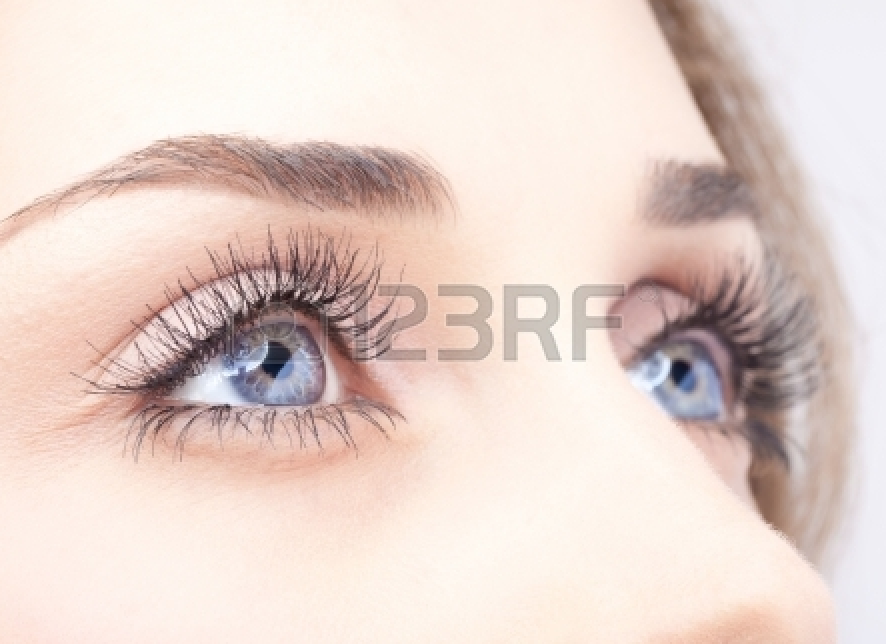
\includegraphics[width=.8\linewidth]{images/beforeHarris.png}
	\caption{Sample image}
	\label{fig:beforeHarris}
\end{minipage}%
\begin{minipage}{.5\textwidth}
	\centering
	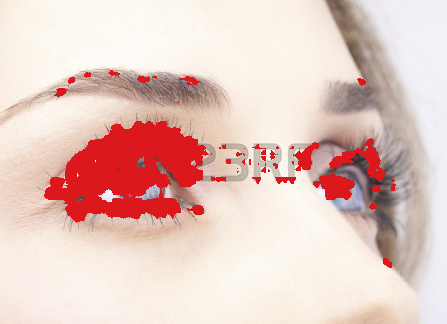
\includegraphics[width=.8\linewidth]{images/afterHarris.png}
	\caption{Harris corner mask applied }
	\label{fig:afterHarris}
\end{minipage}
\end{figure}

As it can be seen from the image, the corner mask centers around the interest points in the image, the eyes and the eyelashes, while leaving the smooth surfaces (the skin) unmarked.

Another observation is that possible watermarks can be present in the image (as seen above), which, of course, the mask detects (they are center pieces of the image, and the corner algorithm cannot determine that they have no real connection with the image).

Furthermore, in some cases the watermark might contain all (or at least a vast majority of) the points in the mask (as seen in Figure~\ref{fig:watermarkHarris}). To avoid such a behavior, I have split the image into 9 sub images (three rows and three columns of identical dimensions) and the Harris mask is applied to each of these.

\begin{figure}[ht!]
\centering
\begin{minipage}{.5\textwidth}
	\centering
	
\includegraphics[width=.8\linewidth]{images/watermarkHarris.png}
	\caption{Single image}
	\label{fig:watermarkHarris}
\end{minipage}%
\begin{minipage}{.5\textwidth}
	\centering
	
\includegraphics[width=.8\linewidth]{images/watermarkHarris9.png}
	\caption{9 subimages}
	\label{fig:watermarkHarris9}
\end{minipage}
\end{figure}

This determines the corner mask to also contain pixels from the center of the image (some of which, unfortunately, are also a watermark).


\subsection{Using SIFT keypoints and descriptors}

As we have seen, the SIFT algorithm computes the keypoints of an image, and then the descriptors of these keypoints. Due to the high similarity nature of our problem, we do not want to compute the keypoints for the entire image, but filter them based on the corner mask determined in the previous section (as observed in Figure~\ref{fig:messiSift} and Figure~\ref{fig:messiCornerSift})

\begin{figure}[ht!]
\centering
\begin{minipage}{.5\textwidth}
	\centering
	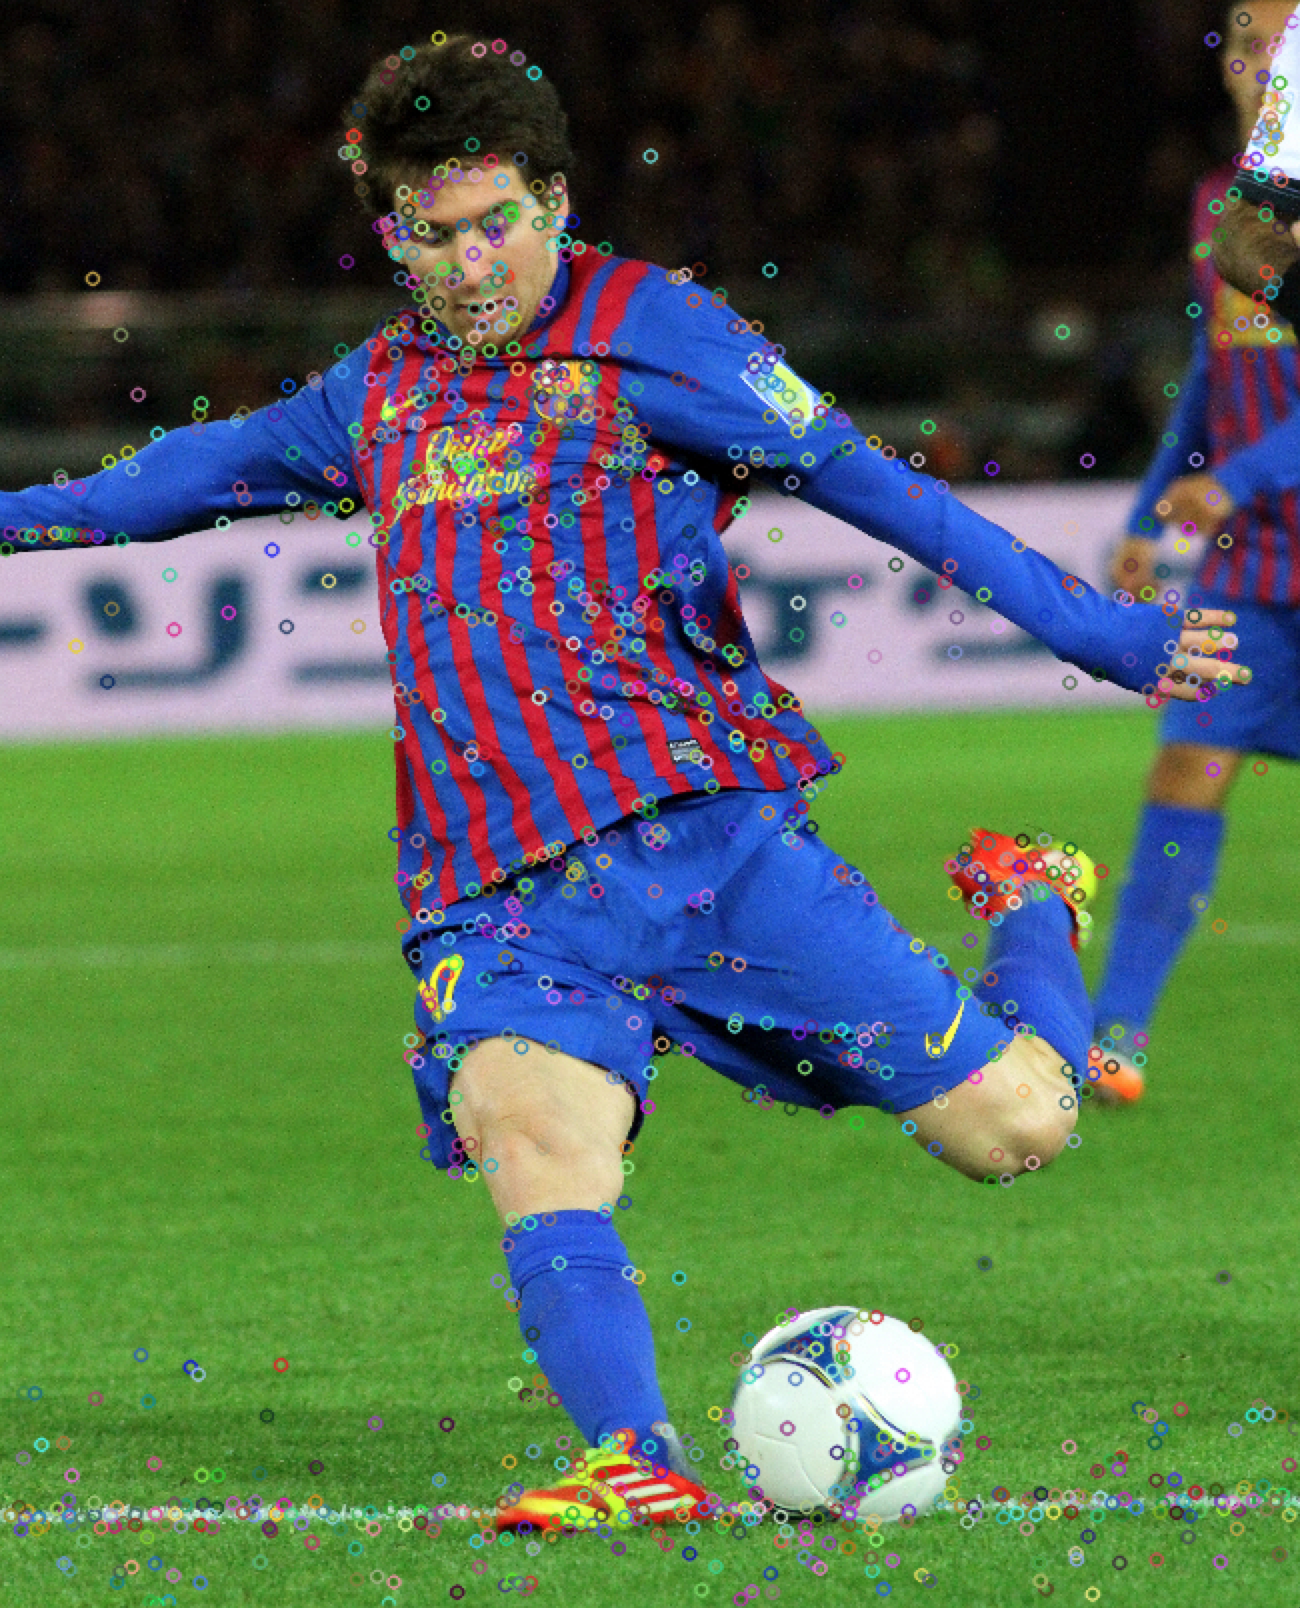
\includegraphics[width=.8\linewidth]{images/messiSift.png}
	\caption{SIFT keypoints for the\\ entire image}
	\label{fig:messiSift}
\end{minipage}%
\begin{minipage}{.5\textwidth}
	\centering
	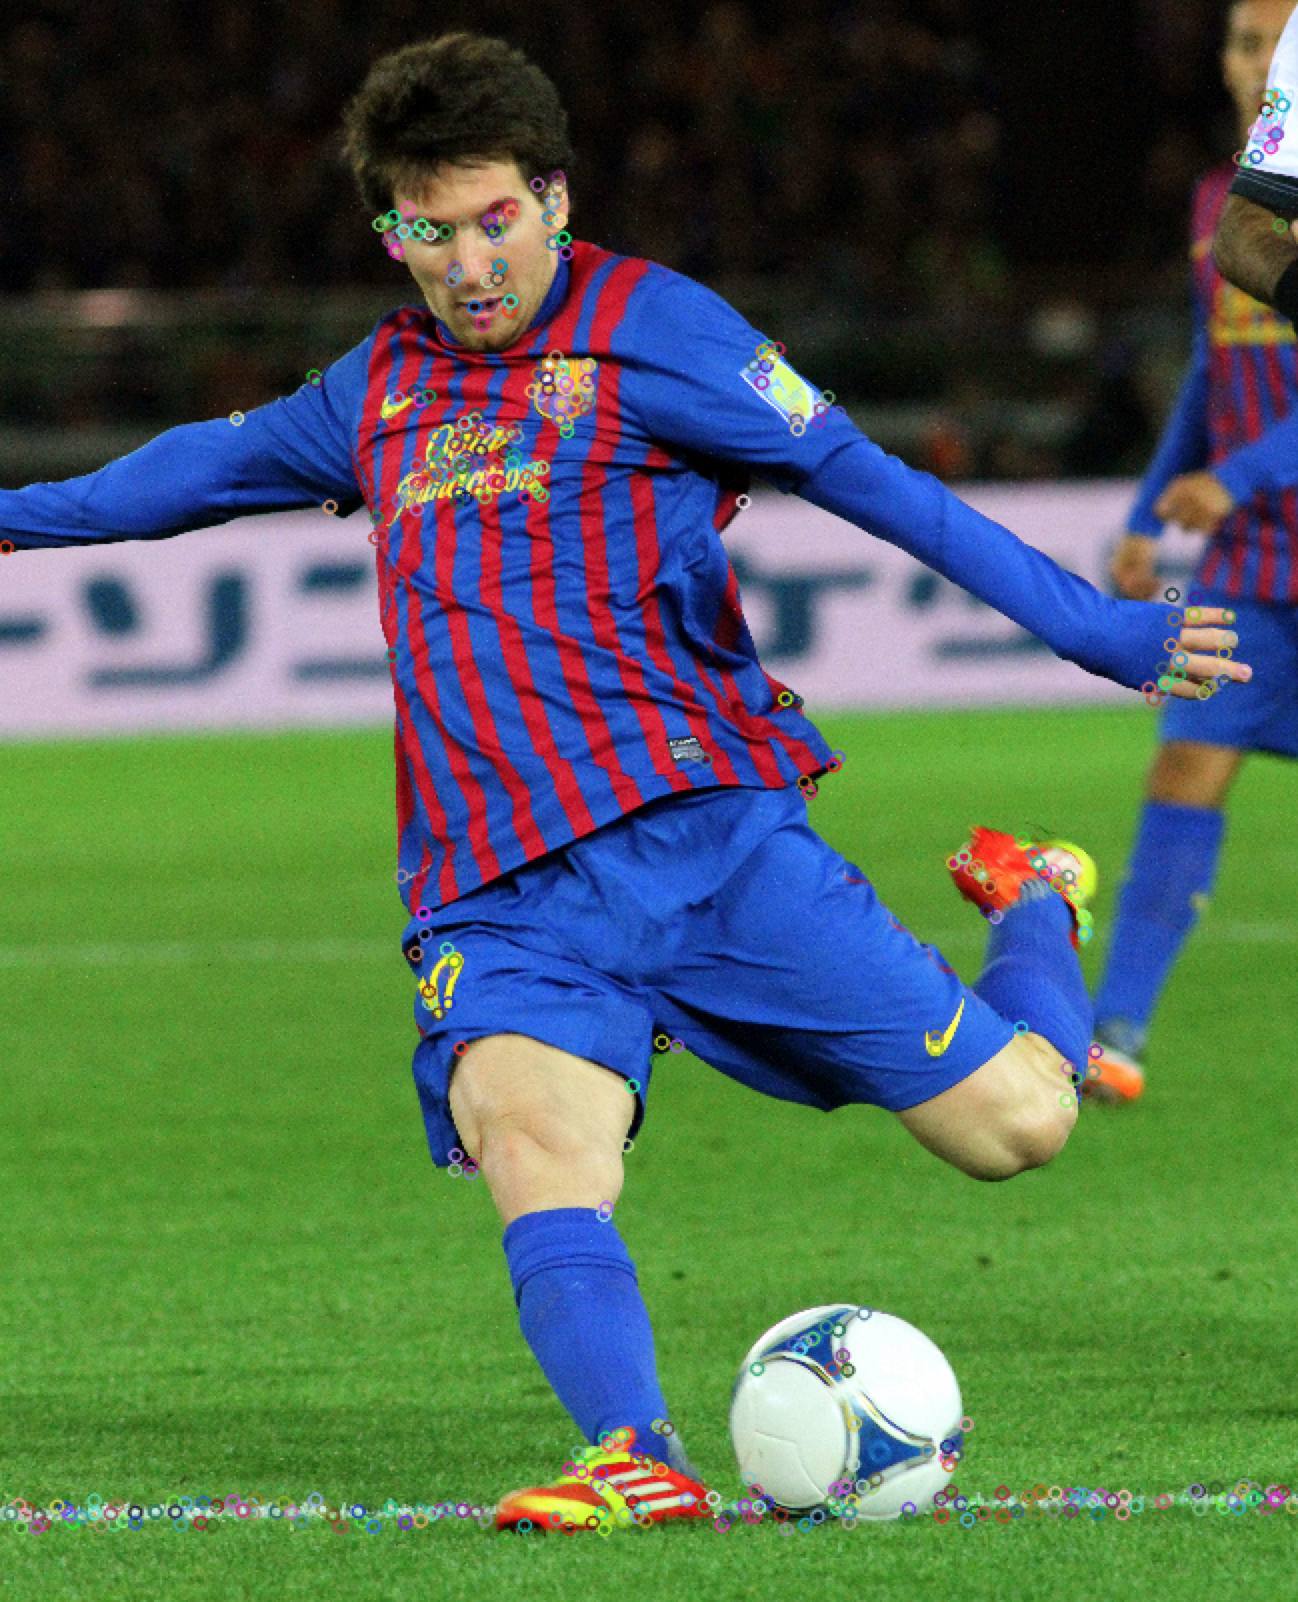
\includegraphics[width=.8\linewidth]{images/messiCornerSift.png}
	\caption{SIFT keypoints for corner mask}
	\label{fig:messiCornerSift}
\end{minipage}
\end{figure}

The SIFT descriptors are then computed for each keypoint located in the corner mask and this will be the information stored for a certain image.

\section{Analysis of a pair of images}

In order to analyze a pair of images, we shall use the SIFT descriptors determined in the previous section. The two sets of descriptors are compared in order to obtain the best matches between pairs of keypoints. A distance is computed between each pair of keypoint descriptors, which is the Euclidian norm between the SIFT descriptors of the keypoints. Experimentally, I have concluded that a match between two keypoints has a high similarity if the Euclidian norm is less than $100$.\\
For a pair of images, we first find the set of corner-mask keypoints and then compute the best matches between these keypoints. We shall keep only the best $10$ matches, and compute the arithmetic mean between the distances of these matches. As stated before, if this mean is smaller than $100$, the two images are considered similar. We shall name this algorithm the $pair\ similarity\ algorithm$.\\
Figure~\ref{fig:compareImages} shows the corresponding matches between two images with two different watermarks, one of which is rotated $90^o$ clockwise.

\begin{figure}[ht!]
\centering
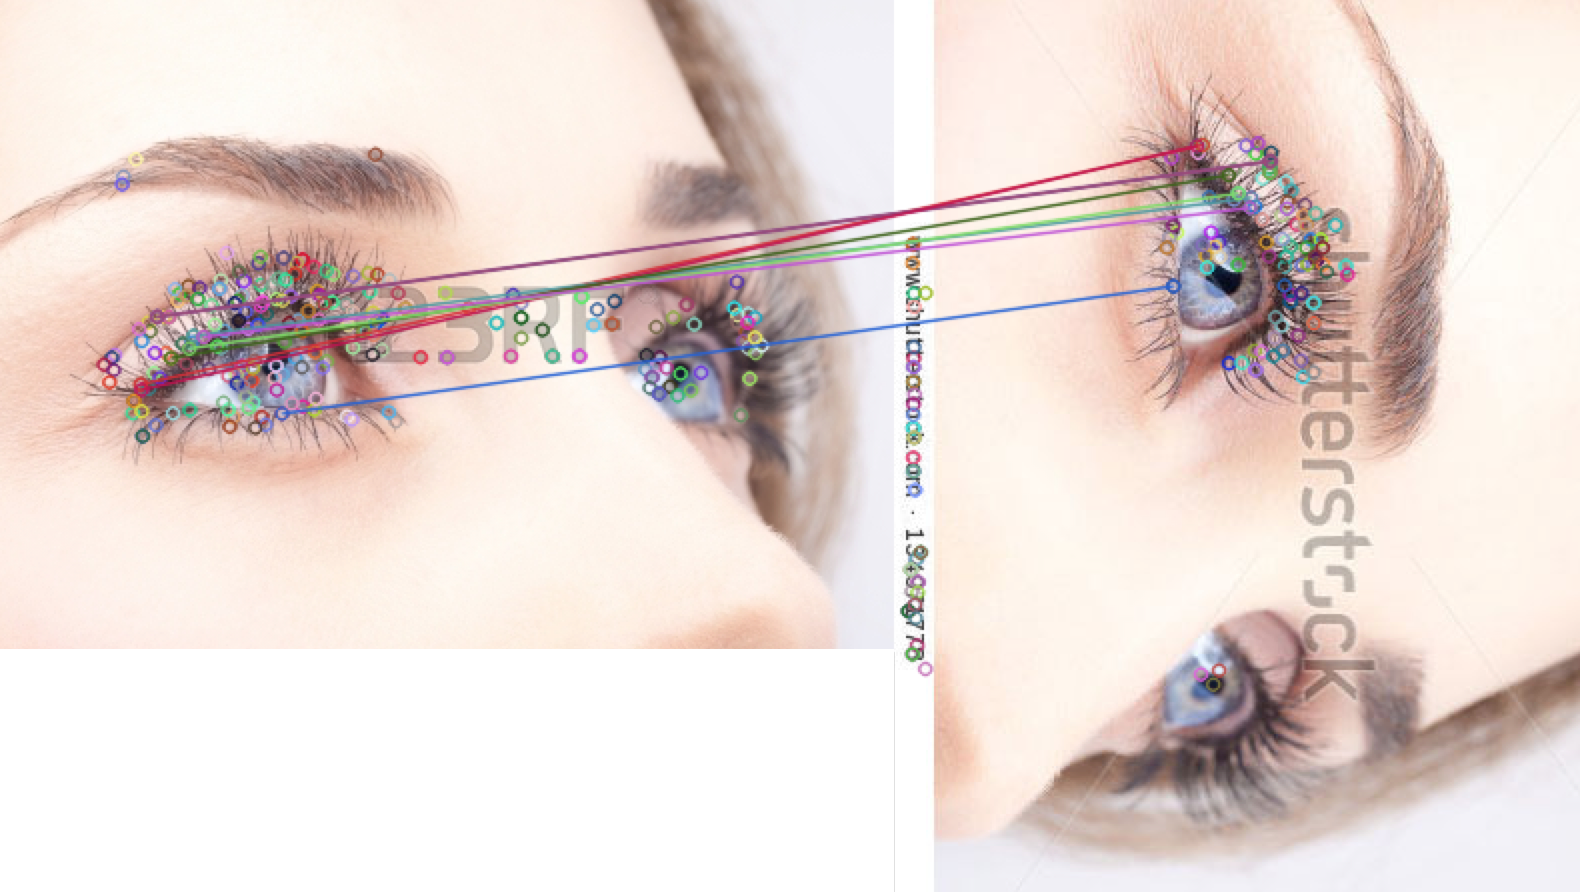
\includegraphics[width=.8\linewidth]{images/compare.png}
\caption{Comparison between two images}
\label{fig:compareImages}
\end{figure}
 
 
\section{Analysis of a set of images}

Suppose that we have a set of images, and we want to compare a test image with the set and detect whether we have a similar image within the set. Of course, the first possibility is the brut force one: we iterate through all the images and apply the $pair\ similarity\ algorithm$ described in the previous section. Although this provides a correct result, it has a complexity of $O(number\_of\_images * image\_match\_time)$. We shall name this basic algorithm as the $linear\ algorithm$. Although this algorithm is very straightforward, its complexity is undesirable if the number of images becomes large. Moreover, most of the images in our set will likely have a big similarity distance with our searched image, so maybe we don't want to apply the full $pair\ similarity\ algorithm$.\\
Thus, we need to determine an efficient algorithm which can filter the initial set of images to a smaller set which contains very likely matching candidates with our test image.\\
The filtering algorithm is implemented as follows: we will maintain a maximum number of $M$ descriptors for each image in the initial set and create a KD-tree with the set of descriptors of the initial images. When a query for a test image arrives, we will compute its descriptors and then perform a $N$ nearest-neighbor search on our KD-tree. Then we will select the top $T$ images with the most descriptors returned by the KD-tree and perform the $linear\ algorithm$. Experimentally, I have determined that the optimal values for $M$, the number of descriptors, $N$, the number of neighbors and $T$, the number of images is $40$, $5$ and $10$. We shall name this algorithm the $kdtree\ algorithm$.
 
 

\chapter{Architecture}
\label{chap:implementation}

\section{Basic structure}

To illustrate the functionality of the described algorithm, we have designed a basic application which maintains a data base of images and, for a given query image, can retrieve the best match between
the query and the image set.\\
The basic structure of the application is shown in Figure~\ref{fig:basicStructure}: all the queries are received by the Load Balancer, which acts like a front end processor and distributes in a round-robin fashion the queries to several Map Reduce servers. When these servers receive a query, they distribute it to the associated Image Servers, which contain the descriptors for various sets of images. The Image Servers compute the top $T$ most similar images and then they send it back to the Map Reducer, which extracts the best images from the received responses and sends them back to the Load Balancer. There are several advantages of separating the Map Reducer from the Load Balancer. First of all, it allows load balancing: the Load Balancer can maintain a queue of requests and the Map Reducer with the least work to do can pick it up and process it. Secondly, it allows different types of Image Servers to be tested, by easily inserting and removing the Image Server module.\\
The querying instance type is not particularly important, it can be either a simple web page or a browser extension (e.g. Google Chrome extension).

\tikzstyle{block3} = [rectangle, draw, fill=blue!20, 
    text width=5.5em, text centered, rounded corners, minimum height=3em]
\tikzstyle{line} = [draw, -latex']
\tikzstyle{cloud} = [draw, ellipse,fill=red!20, node distance=1.5cm,
    minimum height=0.5em]
\tikzstyle{block2} = [rectangle, draw, fill=blue!30, 
    text width=5.5em, text centered, rounded corners, minimum height=4em, node distance=3cm]
\tikzstyle{block1} = [rectangle, draw, fill=blue!50, 
    text width=5.5em, text centered, rounded corners, minimum height=3em]
\tikzstyle{cloud2} = [draw, ellipse,fill=green!50, node distance=1.5cm,
    minimum height=0.5em]

\tikzset{
    %Define standard arrow tip
    >=stealth',
    % Define arrow style
    pil1/.style={
           <-,
           thick,
           shorten <=2pt,
           shorten >=2pt,},
    pil2/.style={
           ->,
           thick,
           shorten <=2pt,
           shorten >=2pt,}, 
}

\begin{figure}[H]
\centering

\begin{tikzpicture}[node distance = 2cm, baseline=1em]
    % Place nodes   
    \node [cloud] (query1) {image query};
    \node [cloud, below of = query1] (query2) {image query};
    \node [cloud, below of = query2] (query3) {image query};
    \node [cloud, below of = query3] (query4) {image query};
    \node [cloud, below of = query4] (query5) {image query};
    \node [block1, right of = query3, node distance = 4cm] (loadbalancer) {Load Balancer};
    \node [block2, right of = loadbalancer, node distance = 3cm] (mapreducer1) {MapReducer};
    \node [block2, below of = mapreducer1] (mapreducer2) {MapReducer};
    \node [block2, above of = mapreducer1] (mapreducer3) {MapReducer};
    \node [block3, right of = mapreducer1, node distance = 3cm] (server1) {Image Server};
    \node [block3, below of = server1] (server2) {Image Server};
    \node [block3, above of = server1] (server3) {Image Server};
    \node [block3, below of = server2] (server4) {Image Server};
    \node [block3, above of = server3] (server5) {Image Server};
    % Draw edges
    \path [line] (query1) -- (loadbalancer);
    \path [line] (query2) -- (loadbalancer);
    \path [line] (query3) -- (loadbalancer);
    \path [line] (query4) -- (loadbalancer);
    \path [line] (query5) -- (loadbalancer);
    \path [line] (loadbalancer) -- (mapreducer1);
    \path [line] (loadbalancer) -- (mapreducer2);
    \path [line] (loadbalancer) -- (mapreducer3);
    \path [line] (mapreducer1) -- (server1);
    \path [line] (mapreducer1) -- (server2);
    \path [line] (mapreducer1) -- (server3);
    \path [line] (mapreducer1) -- (server4);
    \path [line] (mapreducer1) -- (server5);
    
\end{tikzpicture}
\caption{Basic structure of service}
\label{fig:basicStructure}
\end{figure}

\section{Load Balancer}

The Load Balancer acts as a classical server. It uses socket communication in order to receive the queries and send them in a round-robin order to the connected Map Reducers. When a response is received from the Map Reducer the Load Balancer sends it back to the entity that has made the given query.\\

\begin{lstlisting}[language=python, caption=Load Balancer pseudocode]
while (true):
  msg = receiveMessage()
  if msg is a Query:
  	send to next Map Reducer
  else if msg is response from Map Reducer:
  	send response back to querying entity
\end{lstlisting}

The command to run the Load Balancer is:
\begin{lstlisting}[language=bash]
make run_load_balancer PORT_FRONT=10000 PORT_BACK=10001
\end{lstlisting}
where PORT_FRONT is the port on which the queries are received and PORT_BACK is the port on which they are passed along to the Map Reducers.

\section{Map Reducer}

The Map Reducer maintains a set of connections to a number of associated Image Servers to which it broadcasts a received query. The Map Reducer waits for the response from the servers (in the meantime it does not process other queries), and combines the received results, by selecting the images with the highest $image\ pair\ score$ from all the images returned by the Image Servers.\\

\begin{lstlisting}[language=python, caption=Map Reducer pseudocode]
while (true):
  query = receiveQueryFromLoadBalancer()
	
  for server in imageServers:
    send(query, server)
  
  for server in imageServers:
    response = receiveResponse(server)
    allResponses.append(response)
	
  sendToLoadBalancer(top T images from allResponses)
\end{lstlisting}

The command to run the Map Reducer is:
\begin{lstlisting}[language=bash]
make run map_reducer PORT_RECV=10001 PORT_PUB=11000 PORT_RSP=11001 CLIENTS=5
\end{lstlisting}

where PORT_RECV is the same as PORT_BACK from the Load Balancer, PORT_PUB is the port on which the query is transmitted to all Image Servers and PORT_RSP is the port used to receive the responses from the Image Servers.
CLIENTS indicated the number of Image Servers connected to the Map Reducer and, implicitly, how many responses must the Map Reducer wait for after publishing a query.

\section{Image Server}

\subsection{Linear Server}
	The first type of server uses the $linear\ algorithm$ described in \nameref{chap:design}. It stores the list of images that form our database and applies the $linear\ algorithm$ a certain query arrives from the Map Reducer.\\

\begin{lstlisting}[language=python, caption=Linear Image Server pseudocode]
def doLinearProcessing(queryImage, imageList):
  for image in imageList:
    allScores.append(computePairImageScore(queryImage, image))
	
    return allScores.sort()
\end{lstlisting}

\subsection{KD-tree Server}
	The second type of server uses the $kdtree\ algorithm$ described in \nameref{chap:design}. At initialization time the server reads a given list of images from our database, computes its descriptors and applies the above mentioned algorithm when a query arrives from the Map Reducer. The resulting KD-tree is maintained in memory throughout the incoming queries and it it used to find the top $T$ most similar images and return them to the Map Reducer.\\

\begin{lstlisting}[language=python, caption=KD-Tree Image Server pseudocode]
def doKDTreeSearch(queryImage, kdTree):
  filteredImages = kdTree.findNearestNeighbors(queryImage)
	
  return doLinearProcessing(queryImage, filteredImages)
\end{lstlisting}

The main problem when storing the descriptors in the KD-tree is in what form to have the images during the computation. We have three possibilities:
\begin{itemize}
 	\item keep them in the original size
	\item resize all the images to a fixed dimension (eg. $400\times300$)
	\item resize all the images to a fixed width and scale the height
\end{itemize}

\subsubsection{Multi-threaded server}
	In order to support a large number of queries on our service, we have implemented the KD-tree Server as a multi-threaded one, each thread being able to process multiple queries.
	The computation of the KD-tree remains on the main thread and, after it is finished, several threads are created with the purpose of responding to queries from the Map Reducers.\\
	As we mentioned before, the Map Reducer is able to process only one query at a time - it receives a query from the Load Balancer, submits it to the Image Servers, and then waits for the responses from these servers.
	So, to take advantage of the multi-threaded implementation of the Image Servers, we have to create multiple Map Reducers, each of them connected to a certain thread in the Image Servers and able to submit and process queries.\\
	Figure~\ref{fig:threads} shows how to Image Servers with 3 threads interact with 3 Map Reducers.\\

\begin{figure}[ht!]
\centering
\begin{tikzpicture}[node distance = 2cm, baseline=1em]
	\matrix(server1)[draw, matrix of nodes, row sep=0.8cm, inner sep=0.3cm, fill=blue!30] {
		Image Server 1 \\
		\node[block1] (T11) {Thread 1};\\
		\node[block1] (T12) {Thread 2};\\
		\node[block1] (T13) {Thread 3};\\
	};
	\matrix(server2)[draw, matrix of nodes, row sep=0.8cm, inner sep=0.3cm, fill=blue!30,
		below of = server1, node distance = 8cm] {
		Image Server 2 \\
		\node[block1] (T21) {Thread 1}; \\
		\node[block1] (T22) {Thread 2};\\
		\node[block1] (T23) {Thread 3};\\
	};
	\node[block2, left of = server1, node distance = 5cm] (mapreducer1) {Map Reducer};
	\node[block2, below of = mapreducer1, node distance = 5cm] (mapreducer2) {Map Reducer};
	\node[block2, below of = mapreducer2, node distance = 5cm] (mapreducer3) {Map Reducer};
	
	\path[line] (mapreducer1) -- (T11);
	\path[line] (mapreducer1) -- (T21);
	\path[line] (mapreducer2) -- (T12);
	\path[line] (mapreducer2) -- (T22);
	\path[line] (mapreducer3) -- (T13);
	\path[line] (mapreducer3) -- (T23);
\end{tikzpicture}
\caption{Image Servers with 3 threads and associated Map Reducers}
\label{fig:threads}
\end{figure}

\subsection{Multiple KD-trees}

Because of the relative constant time of querying a KD-tree, correlated with the fact that this query is an heuristic one (so the quality of the response may get smaller as the size of the KD-tree grows), we have opted to maintain multiple KD-trees in one KD-tree Image Server. We will use the variable
name $R$ to denote the number of KD-trees per Image Server \\
These KD-trees can be searched in a linear fashion, one at a time, or in parallel, with multiple threads (using OpenMP, for example).\\

\begin{lstlisting}[language=python, caption=Multiple KD-Tree Image Server pseudocode]
def doMultipleKDTreeSearch(queryImage, kdTrees):
	for current_kdTree in kdTrees:
		filteredImages.append(current_kdTree.findNearestNeighbors(queryImage))
	
	return doLinearProcessing(queryImage, filteredImages)
\end{lstlisting}

\subsection{Running the Image Server}

The command used to run an Image Server is:

\begin{lstlisting}[language=bash]
make run_images KEY=data_urls START=0 END=25000 TYPE=linear|kdtree IMAGES_KDTREE=2500 NUM_THREADS=1 PORT_FILE=port_file.json COMP=yes|no
\end{lstlisting}

The parameters are:
\begin{itemize}
	\item KEY: the key in the Redis database which stores the urls to be loaded
	\item START, END: the interval of urls from the KEY to be loaded
	\item TYPE: this can be either $linear$ or $kdtree$ depending on the Image Server type
	\item IMAGES_KDTREE: the number of images per KD-tree: the total number of KD-trees per Image Server is computed as the total number of images (END - START + 1) divided by IMAGES_KDTREE
	\item NUM_THREADS: the number of threads per Image Server
	\item PORT_FILE: a JSON file containing the ports used by each thread for communicating with the associated Map Reducer. An example of port file is listed below, with each two consecutive ports representing a communication channel between a thread and a Map Reducer:\\
\begin{lstlisting}[caption=port_file.json]
  ["11000", "11001", "11100", "11101", "11200", "11201"]
\end{lstlisting}
	\item COMP: this can be either $yes$ or $no$, depending if we want to compute the descriptors for the current images, or if we want to load them from the database
\end{itemize}

\section{Technologies}

The majority of our code, Load Balancer, Map Reducer and Image Serves, is written in C++, because of the high computation nature of our problem. For the image processing and associated algorithm we have used OpenCV version 2.4.8 \cite{opencv}.

\subsection{Image Storing}

At first, we stored all our images in a directory on the hard disk, and we maintained a file with all the names of the images we wanted to load in our Image Servers.
This started to be a problem when the number of images started to grow, because keeping all the images in a single directory increased the access time to the respective files (finding, opening and reading from it).\\

We determined that it is better to store only the urls of the images used in out database (not the actual images), the Image Servers downloading an image whenever they need to use it (at initialization time or at query time). The downloading is done using a CURL library for C++ \cite{libcurl}.\\
Also, to avoid computing the SIFT descriptors for all the images every time we start an Image Server we opted to retain those descriptors in our database, and only load them when needed.\\
We maintain a Redis server \cite{redis} on a machine which stores all the urls and the descriptors of the images, and which we can query using a specific C++ library.

\subsection{Process Communication}

For the process communication, we opted to use sockets so that the various servers can reside on different machines. ZeroMQ sockets \cite{zeromq} looked liked the best option, because of their robustness, small running time, auto-handling of connection failures and multiple types.\\
The ZeroMQ sockets that we used in our service are:
\begin{itemize}
	\item ROUTER-DEALER. We used this pair of sockets to implement the Load Balancer. The ROUTER socket can accept multiple connections, add a header to the message, to remember which of the connected clients sent it and forwards it to the DEALER.\\
	The DEALER receives the messages from the ROUTER and distributes them in a round-robin fashion to all the connected clients (which in fact are the Map Reducers). When a reply comes to the DEALER, it forwards it to the ROUTER, which, by inspecting the message's header, identifies the original client and sends it back.
	\item REP. The Map Reducer maintains this type of socket in its communication with the Load Balancer. It allows consecutive operations of receive and send, which suits very well our "receive query - send answer" protocol
	\item PUB-SUB. This pair of sockets forms the connection between a Map Reducer and its associated Image Servers.
	The PUB (publish) socket sends it message to all SUB (subscribed) sockets, making it ideal for the process of map reducing.
	\item PULL-PUSH. This pair of sockets implements the response communication between the Image Server and the Map Reducer. The PUSH (Image Server) sends its response, and the PULL (Map Reducer) receives it.
\end{itemize}

\subsection{Submitting a query and image retrieval}

For submitting a query, we use a JSON-encoded string, which is sent via socket communication to the LoadBalancer, which then forwards it in the above mentioned way. An example of a JSON query string is given below:

\begin{lstlisting}[caption=Query JSON]
{
  "name" : "http://webpa-mp:8080/image/98070.jpg",
  "num_responses" : 10,
  "type_experiment" : 0
}
\end{lstlisting}

The $name$ key represents a url with an associated image, the $num\_responses$ key represents the number of similar images which we want to be returned, and the $type\_experiment$ key represents one of the 3 metrics used (described in \nameref{chap:design}) to be used for extracting the images from the KD-tree.\\

A JSON response string is shown below:

\begin{lstlisting}[caption=Response JSON]
{
  "name": "http://webpa-mp:8080/image/141579.jpg http://webpa-mp:8080/image/223221.jpg http://webpa-mp:8080/image/116303.jpg http://webpa-mp:8080/image/265219.jpg http://webpa-mp:8080/image/216601.jpg http://webpa-mp:8080/image/100891.jpg",
  "scores": "0 18 22 51 79 200 ",
  "time": 1.25,
  "num_responses": 10,
  "type_experiment": 0
}
\end{lstlisting}

The $name$ filed now contains the list of similar images, $scores$ the associated $pair\ image\ scores$ and $time$ the time of the query on the KD-trees The coding and decoding of JSON arrays is done using a special C++ library \cite{jsoncpp}.

\subsection{Web Server}

For the purpose of a web server, which we need for the submission of the queries and local image retrieval, we have used WebPY \cite{webpy}. This server hosts our local images - which can be retrieved by accessing a certain URL, and also is responsable for receiving the queries, forwarding them to the Load Balancer and then generating the HTML for the result page.

\subsection{User interface}

For testing purposes, we have implemented a Google Chrome extension \cite{chromeExtension} which allows a user to select an image from his browser, right click on it, and search our database for similar images. An example of such a search is shown below, where we want to find similar images of the pirate-skull image from the top-right corner: \\

\begin{figure}[ht!]
\centering
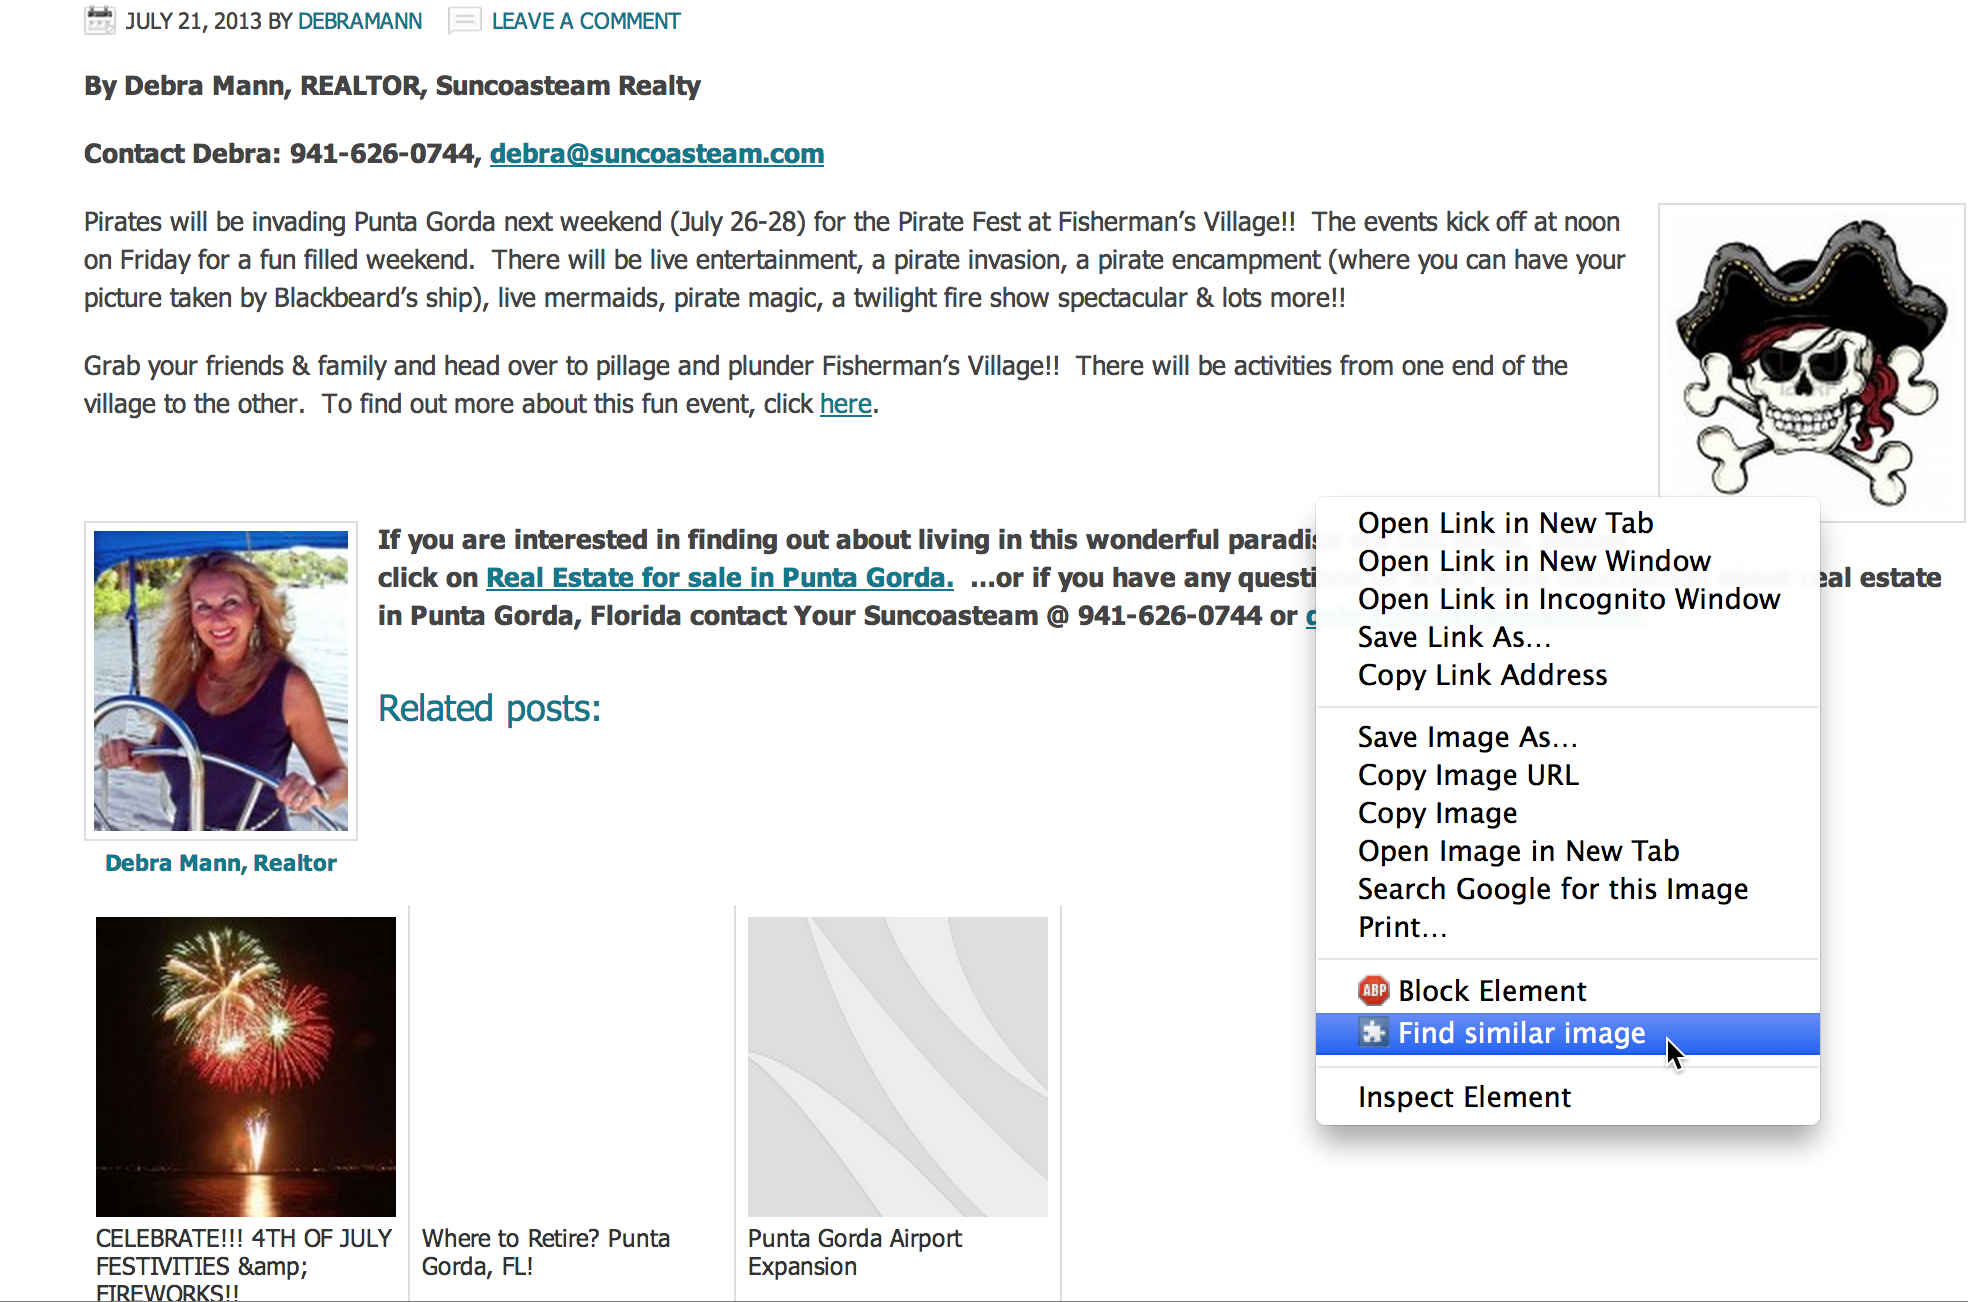
\includegraphics[width=.9\linewidth]{images/extension.png}
\caption{Using the Google Chrome extension}
\end{figure}

The results from the image search can be seen below, where we have the top 3 most similar images from our database, along with the total query time and the associated $pair\ image\ scores$. We have considered a score of less than $50$ represents a highly similar image (marked by a green color), a score less than $100$ a possible similar image (marked by an orange color) and a score higher than $100$ an improbable match (marked with red). 

\begin{figure}[ht!]
\centering
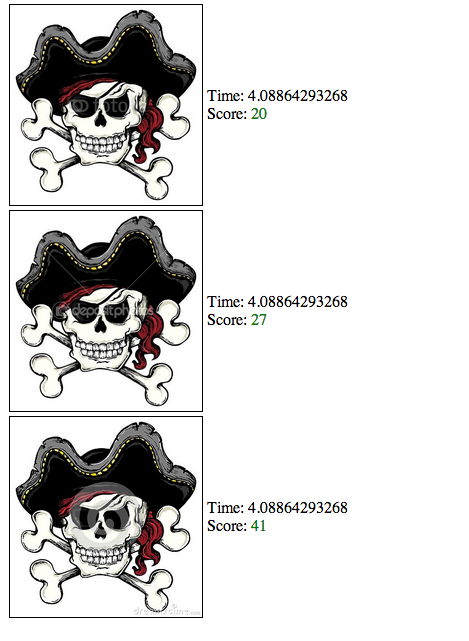
\includegraphics[width=.5\linewidth]{images/extensionResult.png}
\caption{Google Chrome extension result}
\end{figure}


The overall architecture of the entire system is shown in the Figure~\ref{fig:architecture}.
The general workflow of the application is:
\begin{enumerate}
	\item The querying instance (Google Chrome extension) sends the query to the web.py server
	\item The server redirects the query to the Similar Image Service
	\item The service gets the URLs and descriptors from the database
	\item The service may attempt to download images from the web.py server
	\item The server generates the result page, with the found images
\end{enumerate}

\begin{figure}[ht!]
\centering

\begin{tikzpicture}[node distance = 2cm, baseline=1em]
		\node[cloud2] (chrome) {Chrome Extension};
		\node[block2, above of = chrome, node distance = 5cm] (server) {web.py Server}
			edge[pil1] node[auto] {1. Similar Image Query} (chrome.north) ;
		\node[block1, right of = server, node distance = 6cm] (service) {Similar Image Service}
			edge[pil2, bend right = 45] node[auto] {4. Get Images} (server.north) 
			edge[pil1, bend left = 45] node[auto] {2. Send Query} (server.south) ;
		\node[block1, left of = server, node distance = 6cm] (html) {HTML Result Page}
			edge[pil1] node[auto] {5. Show Results} (server.west);
		\node[block1, below of = service, node distance = 7cm] (db) {Redis Database}
			edge[pil1] node[auto] {3. Get URLs and/or descriptors} (service.south);
\end{tikzpicture}
\caption{System architecture}
\label{fig:architecture}
\end{figure}



\chapter{Results}

I have tested the two algorithms described in \nameref{chap:design} using the structure given in \nameref{chap:implementation}.\\
There are two major parts which should be analyzed: the correctness of the algorithm and its running time.

\section{Correctness}

We have collected a set of $4500$ images from the Internet, which we have classified in about $1600$ similarity sets, each set being composed of up to five images. The images within a similarity set differ in size, having various watermarks and filters applied (these sets are known to be correct beforehand). We have inserted these images in a larger set of $100.000$ images taken from the Internet and performed queries for each of the $4500$ images of the similarity sets, getting the top $10$ similar images. We want to observe:
\begin{itemize}
	\item if the algorithm finds the exact match, i.e. the image that has been queried with
	\item if the algorithm finds the other images which are part of the same similarity set
	\item the mean running time of a query
	\item how varying the metrics described in \nameref{chap:design} above influences the results of the query
\end{itemize}

We evaluate the response to a query, by looking at the indices of the images from the current similarity set in the list of results returned by the query. Thus, the $index\ score$ for a certain query can be computed as the sum of these indices; the smaller the sum, the closer in the response list are the images we want to find. \\
For the set of $100.000$ images we use $P=20$ KD-trees, each KD-tree storing the descriptors for $N=5000$ images. The descriptors are computed for images which are resized to keep the aspect ratio (the third storing possibility described in \nameref{chap:implementation}).\\

The results of this test can be seen in the following two tables. The first one describes, for similarity sets of size $3$, $4$ and $5$, and for the metrics described in \nameref{chap:design}, the average number of how many of these images are found in the list of $10$ returned images.\\

\begin{table}[H]
\centering
\begin{tabular} {c | c | c | c}
	& max nr descs & min avg & max dist to avg \\
	\hline
	3 & 2.85 & 2.63 & 2.86 \\
	\hline
	4 & 3.85 & 3.55 & 3.85 \\
	\hline
	5 & 4.65 & 4.13 & 4.64 \\
\end{tabular}
\caption{Average number of found images for $P=20$ and $N=5000$}
\end{table}

The second table shows the $index\ score$ (described above) for the same queries and metrics.\\

\begin{table}[H]
\centering
\begin{tabular} {c | c | c | c}
	& max nr descs & min avg & max dist to avg \\
	\hline
	3 & 4.86 & 6.85 & 4.78 \\
	\hline
	4 & 7.87 & 10.24 & 7.85 \\
	\hline
	5 & 13.47 & 17.48 & 13.35 \\
\end{tabular}
\caption{$Index\ scores$ for $P=20$ and $N=5000$}
\end{table}

It can be observed that the third metric, the largest distance from the descriptors of an image to the average of all found descriptors, provides the best results.\\

\subsection{Fixed dimension image storing}
	We computed the descriptors for images resized to a fixed value (height $400$ and width $300$), and analyzed the same metrics and scores described above. The results can be seen in tables
\ref{table:fixDimension1} and \ref{table:fixDimension2}. These results confirm that this image storing
performs worse than the aspect-ratio one, so we have decided to continue using the first one.\\
	 
\begin{table}[H]
\centering
\begin{tabular} {c | c | c | c}
	& max nr descs & min avg & max dist to avg \\
	\hline
	3 & 2.69 & 2.08 & 2.73 \\
	\hline
	4 & 3.55 & 2.60 & 3.62 \\
	\hline
	5 & 4.17 & 2.80 & 4.32 \\
\end{tabular}
\caption{Average number of found images for $P=20$, $N=5000$ and fix dimension storing}
\label{table:fixDimension1}
\end{table}

\begin{table}[H]
\centering
\begin{tabular} {c | c | c | c}
	& max nr descs & min avg & max dist to avg \\
	\hline
	3 & 6.32 & 11.93 & 5.97 \\
	\hline
	4 & 10.37 & 18.46 & 9.84 \\
	\hline
	5 & 16.8 & 28.35 & 15.67 \\
\end{tabular}
\caption{$Index\ scores$ for $P=20$, $N=5000$ and fix dimension storing}
\label{table:fixDimension2}
\end{table}

\subsection{Varying the number of images per KD-tree}

We also wanted to see how the number of images within a KD-tree influences the above metrics,
so we separated the $100.000$ images into $P=40$ KD-trees, each of them storing $2500$ images.
We applied the same correctness test described above, the average number of found images and the $index\ score$ is shown in the tables below.\\

\begin{table}[H]
\centering
\begin{tabular} {c | c | c | c}
	& max nr descs & min avg & max dist to avg \\
	\hline
	3 & 2.87 & 2.64 & 2.88 \\
	\hline
	4 & 3.82 & 3.55 & 3.84 \\
	\hline
	5 & 4.65 & 4.13 & 4.66 \\
\end{tabular}
\caption{Average number of found images for $P=40$ and $N=2500$}
\end{table}

\begin{table}[H]
\centering
\begin{tabular} {c | c | c | c}
	& max nr descs & min avg & max dist to avg \\
	\hline
	3 & 4.83 & 6.80 & 4.81 \\
	\hline
	4 & 8.20 & 10.41 & 8.04 \\
	\hline
	5 & 13.4 & 17.32 & 13.4 \\
\end{tabular}
\caption{$Index\ scores$ for $P=40$ and $N=2500$}
\end{table}

As it can be seen, a smaller number of images per KD-tree provides a higher quality response, which is what we expected, due to the high multi-dimensionality of our problem (a descriptor is composed out of $128$ numbers).
For the overall algorithm, we will have to determine the optimum number of images per KD-tree, in order to strike a balance between the total number of processes and the quality of the response.\\

\subsection{Single KD-tree analysis}

Also, we have constructed a single KD-tree which contains the $4500$ images from the similarity set in order to test the three different metrics described in \nameref{chap:design} for selecting the filtered images.\\
We retained the $image\ pair\ score$ of the returned similar images, and evaluated these three metrics by computing the following $correctness\ scores$:
\begin{itemize}
	\item the mean between the $image\ pair\ scores$
	\item the sum of the differences between the $pair\ scores$ of two consecutive similar images in the returned list
	\item the maximum $image\ pair\ score$
\end{itemize}
The goal is to minimize each of these $correctness\ scores$.
The results of this test are shown in Table \ref{table:correctness}:\\

\begin{table}[H]
\centering
\begin{tabular} {c | c | c | c}
	& max nr descs & min avg & max dist to avg \\
	\hline
	mean & 661880 & 693745 & 647355 \\
	\hline
	sum of diff & 867877 & 1021543 & 856521 \\
	\hline
	max score & 1162618 & 1134470 & 1150899 \\
\end{tabular}
\caption{$Correctness\ scores$ for KD-tree with $N=4500$}
\label{table:correctness}
\end{table}

As it can be seen, the third metric, largest distance from the descriptors of an image to the average of all found descriptors, performs the best out of the three metrics.\\

\subsection{Multiple KD-trees in an Image Server}

As stated in \nameref{chap:implementation}, we decided to maintain multiple KD-trees in one Image Server in order to improve the quality of the heuristic search on one such KD-tree and reduce the total number of processes.\\
On the same set of $100.000$ images, we created $P=40$ Image Servers, with each server having $5000$ images and $R=2$ KD-trees (that means $N=2500$ images per KD-tree), so that we could compare the $correctness\ scores$ between this implementation and the one with $R=1$.\\
These are shown in the tables below:\\

\begin{table}[H]
\centering
\begin{tabular} {c | c | c | c}
	& max nr descs & min avg & max dist to avg \\
	\hline
	3 & 2.86 & 2.5 & 2.89 \\
	\hline
	4 & 3.83 & 3.35 & 3.86 \\
	\hline
	5 & 4.6 & 4.75 & 4.66 \\
\end{tabular}
\caption{Average number of found images for $P=40$, $N=2500$ and $R=2$}
\end{table}

\begin{table}[H]
\centering
\begin{tabular} {c | c | c | c}
	& max nr descs & min avg & max dist to avg \\
	\hline
	3 & 4.76 & 8.03 & 4.67 \\
	\hline
	4 & 7.96 & 11.92 & 7.78 \\
	\hline
	5 & 13.56 & 20.35 & 13.49 \\
\end{tabular}
\caption{$Index\ scores$ for $P=40$, $N=2500$ and $R=2$}
\end{table}

It can be seen that the scores are comparable with the ones obtained from running the algorithm it the two cases shown in the previous subsections, so it can be confirmed that using multiple KD-trees of a fixed (and lesser size) is in our advantage when the overall dataset becomes larger, in order to avoid a large number of Image Servers.
 
\subsection{Internet Search}

Besides running the algorithm on our similarity sets, we also took some images from our $100.000$ set and used Google Image Search or TinEye to find replicas of those images on the Internet. Then we did a reverse search of those images with our algorithm to see if it finds the original images used in the query.\\
We had some interesting results, shown in Figure~\ref{fig:example1.1} and Figure~\ref{fig:example2.1}.\\

\begin{figure}[ht!]
\centering
\begin{minipage}{.5\textwidth}
	\centering
	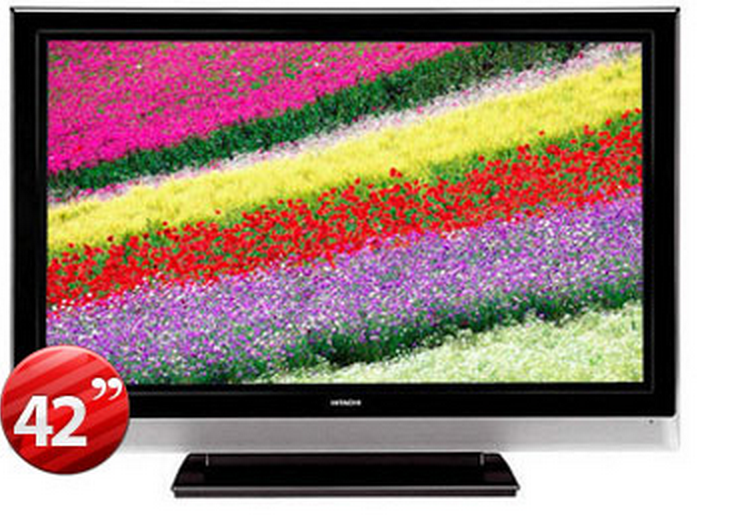
\includegraphics[width=.8\linewidth]{images/fieldSite.png}
	\caption{Image from website}
	\label{fig:example1.1}
\end{minipage}%
\begin{minipage}{.5\textwidth}
	\centering
	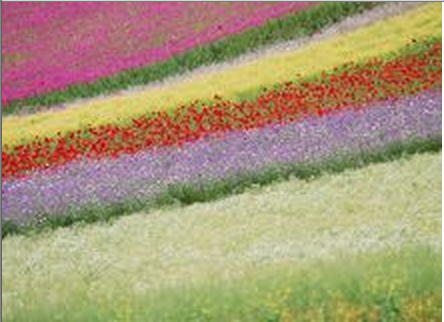
\includegraphics[width=.8\linewidth]{images/field.png}
	\caption{Image from database}
\end{minipage}
\end{figure}

\begin{figure}[ht!]
\centering
\begin{minipage}{.3\textwidth}
	\centering
	
\includegraphics[width=.8\linewidth]{images/pumpkinSite.png}
	\caption{Image from\\ website}
	\label{fig:example2.1}
\end{minipage}%
\begin{minipage}{.3\textwidth}
	\centering
	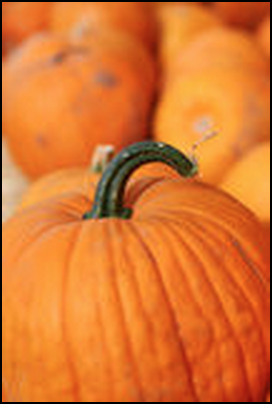
\includegraphics[width=.8\linewidth]{images/pumpkin.png}
	\caption{Image from database}
\end{minipage}
\end{figure}

\section{Running Time}
We have tested our algorithm on a machine with 55GB of RAM, 16 quad-core processors with a frequency of 2.4GHz.\\

\subsection{Comparison between $kdtree\ algorithm$ and $linear\ algorithm$}
The first experiment that we did was comparing the runtimes of the $linear\ algorithm$ with the $kdtree\ algorithm$ by running them on sets of $5, 10, 20, 50, 200, 350$ and $500$ images. The corresponding running times are shown in Figure~\ref{fig:runtimesBasic}.\\
The red line shows the corresponding running times for the $linear\ algorithm$, while the green one shows the times for the $kdtree\ algorithm$. As it can be seen, the $kdtree\ algorithm$ outperformes the linear one, with the same returned image (so it does not give different results). The non-ascending running times of the $kdtree\ algorithm$ can be explained by the fact that the KD-tree data structure is traversed heuristically, so depending on the given input a certain query can execute with varying running times. For a KD-tree of $5000$ images and $5000$ queries, the mean running time of a nearest-neighbor search is $1.36$ seconds.\\
Of course, the $kdtree\ algorithm$ does require an initialization time, which is the price that has to be paid in order to perform fast queries. Figure~\ref{fig:totalRuntimes} shows the sum between the initialization time and query time of a linear image server and an image server which constructs a KD-tree. As it can be seen, the initialization time for the KD-tree grows linearly, but this gets compensated by the small query time. For a $500$-size image set, the initialization and a query on the KD-tree takes $36.771$ seconds, which is less than a query on the same image set using the $linear\ algorithm$, which takes $77.331$ seconds.

\begin{figure}[ht!]
\centering
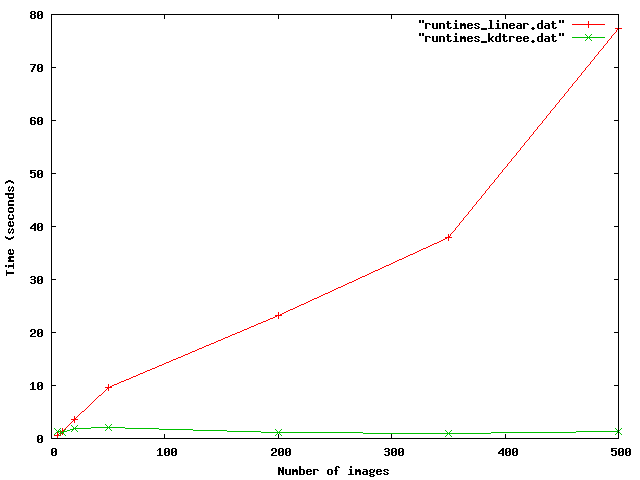
\includegraphics[width=.7\linewidth]{images/runtimesBasic.png}
\caption{Query runtime of the two algorithms}
\label{fig:runtimesBasic}
\end{figure}

\begin{figure}[ht!]
\centering
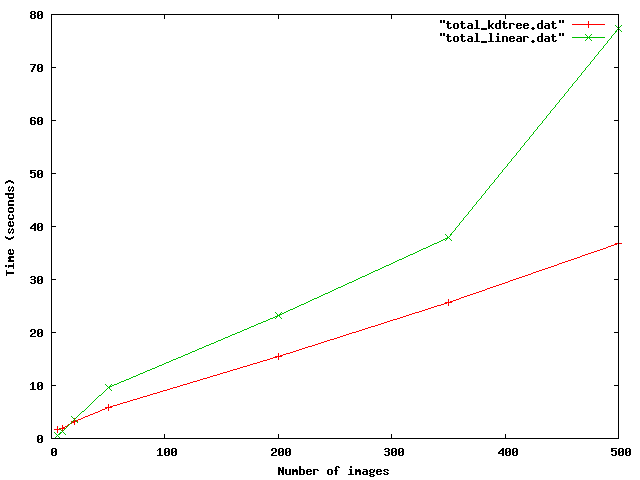
\includegraphics[width=.7\linewidth]{images/totalRuntimes.png}
\caption{Total init and query time for $linear\ algorithm$ and $kdtree\ algorithm$}
\label{fig:totalRuntimes}
\end{figure}

\begin{table}
\centering
\begin{tabular} {c | c | c}
	number of images & $linear\ algorithm$ time & $kdtree\ algorithm$ time \\
	\hline
	5 & 0.60 & 1.391 \\
	10 & 1.23 & 1.21 \\
	20 & 3.54 & 1.90 \\
	50 & 9.58 & 2.08 \\
	200 & 23.28 & 1.05 \\
	350 & 38.00 & 0.96 \\
	500 & 77.33 & 1.39 \\
\end{tabular}
\caption{Query runtime}
\end{table}

\begin{table}
\centering
\begin{tabular} {c | c }
	number of images & $kdtree\ algorithm$ time \\
	\hline
	5 & 1.68 \\
	10 & 1.81 \\
	20 & 3.24 \\
	50 & 5.80 \\
	200 & 15.51 \\
	350 & 25.58 \\
	500 & 36.77 \\
\end{tabular}
\caption{Init and query runtime}
\end{table}



\subsection{Large scale KD-trees}

The second set of tests have been concentrated on analyzing the behavior of large scale KD-trees.
As stated above, our main concern was the initialization time of a KD-tree, which is divided into two steps: the computation of the descriptors for the images, and the construction of the actual KD-tree.\\
In Figure~\ref{fig:totalInit} we can see the total initialization time for a KD-tree, and the time needed only for the construction of the KD-tree data structure (presuming that the descriptors are already computed). \\
\begin{figure}[ht!]
\centering
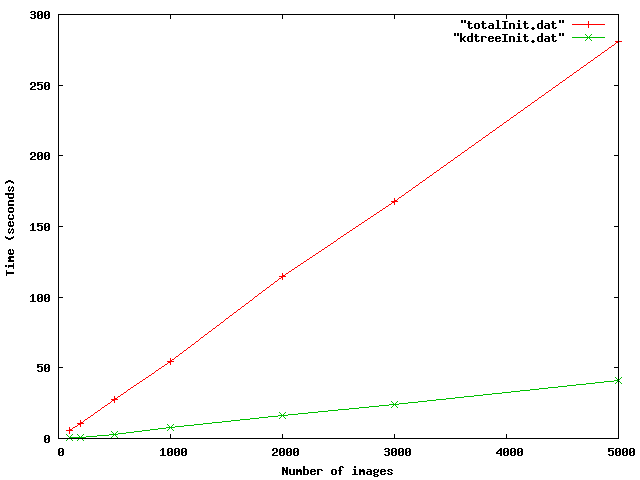
\includegraphics[width=.8\linewidth]{images/totalInit.png}
\caption{Initialization runtimes}
\label{fig:totalInit}
\end{figure}

\begin{table}[H]
\centering
\begin{tabular} {c | c | c}
	number of images & total init (seconds) & kdtree init (seconds) \\
	\hline
	100 & 5.34 & 0.48 \\
	200 & 10.53 & 0.99 \\
	500 & 27.71 & 3.17 \\
	1000 & 54.52 & 7.72 \\
	2000 & 114.27 & 16.26 \\
	3000 & 167.83 & 24.31 \\
	5000 & 280.67 & 41.20 \\
\end{tabular}
\caption{Descriptor computation and KD-tree init time}
\end{table}

Because the total number of images is divided into KD-trees of fixed dimension (in our case $5000$ images), inserting a new image into our database is constant, because it just implies creating a new KD-tree (or expanding a current one, if its dimension doesn't exceed $5000$ images).\\

\subsection{Multiple KD-tree servers}

As shown above, the running time of a nearest-neighbor search is constant, due to its heuristic nature, the overall query time varies depending on the number of processes involved in the search.
This is due to the increasing socket communication between the Map Reducer and the growing number of processes.
We illustrate this overall running time in Figure~\ref{fig:overallTime}, where each process holds a KD-tree of $1000$ images (a higher number of images would not have influenced the process). For each number of processes $20$ queries have been run and the mean execution time of them is listed in table \nameref{table:processTime}, as well as in the figure.\\

\begin{table}[H]
\centering
\begin{tabular} {c | c}
	number of KD-tree servers & query time (seconds) \\
	\hline
	5 & 2.85\\
	10 & 3.24\\
	20 & 3.53\\
	40 & 5.50\\
	60 & 6.38\\
	80 & 8.23\\
	100 & 8.74\\
\end{tabular}
\caption{Execution time for increasing number of KD-tree servers}
\label{table:processTime}
\end{table}

\begin{figure}[H]
\centering
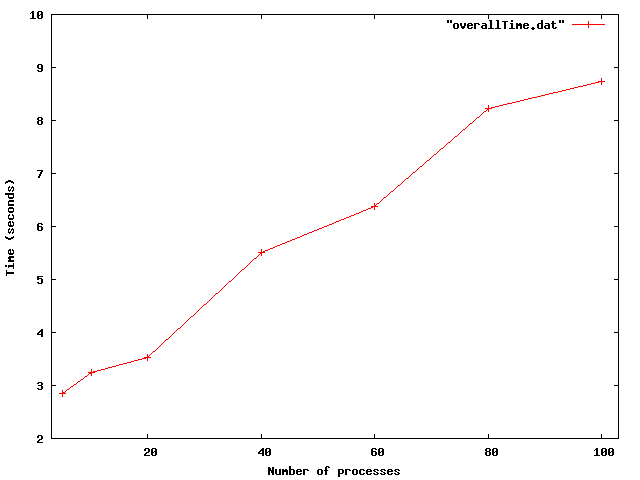
\includegraphics[width=.8\linewidth]{images/overallTime.png}
\caption{Overall query times}
\label{fig:overallTime}
\end{figure}

\subsection{Multi-threaded servers}

As stated in \nameref{chap:implementation}, in order to be able to handle a large number of queries at the same time, the KD-tree servers are multi-threaded, with each separate thread being connected to a different Map Reducer and, thus, being able to support multiple queries simultaneously.\\
Table \ref{table:threadTime} shows the running time for a number of $10$ KD-tree servers, each with $2500$ images and respective number of threads and queries.\\
It can be easily observed that there is a big running time improvement when the number of queries gets bigger and the number of threads increases. In the case of a smaller number of queries, a bigger number of threads does not improve the running time, partially because of the overhead caused by the creation of multiple threads and the overhead of multiple Map Reducers and synchronization between them. \\
Also, because a service with a large number of images will have a considerable amount of Image Servers running (and, implicitly, number of processes), creating more threads will certainly increase the load of the system and not have the desired effect.\\
Inside an Image Server, the KD-tree structure is shared between processes, so, during multiple queries done by multiple threads, the nearest neighbor search performed on the KD-tree may be
a computational bottle neck, all the threads accessing the same data structure.
To avoid this, in case we use multiple KD-trees inside the same Image Server, it could be a good idea to perform the nearest neighbor search in a random order, thus time-multiplexing the access to the data structures.\\

\begin{table}[H]
\centering
\begin{tabular} {c | c | c | c | c}
	\backslashbox{number\\ of threads}{number of\\ queries} & 20 & 50 & 100 & 200 \\
	\hline
	1 & 74.13 & 176.28 & - & - \\
	2 & 38.28 & 94.77 & - & - \\
	3 & 28.15 & 77.51 & - & -\\
	5 & 23.81 & 57.04 & 95.90 & 217.64\\
	10 & - & - & 91.43 & 183.12 \\
	20 & - & - & 90.23 & 180.20 \\
\end{tabular}
\caption{Running time (seconds) for a given number of processes and queries}
\label{table:threadTime}
\end{table}

\subsection{Multiple KD-trees per Image Server}

We analyzed how a certain KD-tree Image Server with a varying number of linear processed KD-trees performs when submitting a query, in order to determine a viable value for the $R$ parameter (the number of KD-trees that form a KD-tree Image Server).\\
In Figure~\ref{fig:multipleKDTrees} and in Table \ref{table:multipleKDTrees} we can observe the running time per query as we increase the number of KD-trees for with $N=2500$ images.\\

\begin{table}[H]
\centering
\begin{tabular}{c | c}
	$R$, number of KD-trees & running time (seconds) \\
	\hline
	2 & 2.45 \\
	3 & 2.75 \\
	5 & 2.84 \\
	10 & 3.01 \\
	20 & 3.44 \\
	40 & 4.41 \\
\end{tabular}
\caption{Running time with various number of KD-trees per KD-tree Image Server}
\label{table:multipleKDTrees}
\end{table}

\begin{figure}[H]
\centering
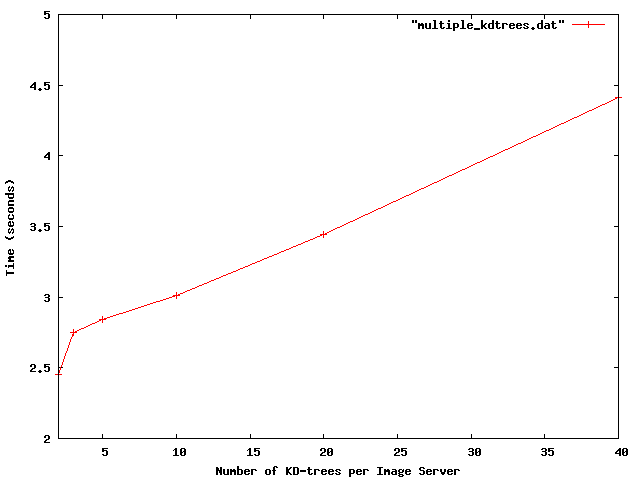
\includegraphics[width=.8\linewidth]{images/multipleKDTrees.png}
\caption{Running time with various number of KD-trees per KD-tree Image Server}
\label{fig:multipleKDTrees}
\end{figure}

By looking at these running times, we can determine that we can easily increase the number of KD-trees per Image Server, as long as we maintain a decent number of images as input for the $linear\ algorithm$, which is used after the actual KD-tree search.\\

\section{Interpretation of results}

By looking both at the running time and correctness of the algorithm, along with the varied parameters which compose it, we have determined the best way to run it when handling a large amount of images:
\begin{itemize}
	\item store images maintaining aspect ratio
	\item store beforehand the computed image descriptors
	\item use the third metric for extracting images from KD-trees: "the images with the largest distance between its descriptors and the average of all found descriptors (from all the images)"
	\item keep a relatively small number of Image Servers
	\item keep a moderate number of threads per Image Server, especially if there isn't a large number of queries
	\item increase the number of KD-trees per Image Server
\end{itemize}


\chapter{Conclusions}

In this paper we have developed a scalable algorithm for finding similar images in a large database, using the Harris corner transformation, the SIFT descriptors and multiple KD-trees for storing the image data.\\
We have designed a basic architecture for our service, consisting of a back-end side, formed by a Load Balancer, multiple Map Reducers and Image Servers, and a front-end side, represented by a Google Chrome extension.\\
We have explored several metrics for selecting images out of the KD-trees and have analyzed how these different metrics influence the images returned by a query.\\
We have analyzed the running time of the algorithm, varying the dimensions of the image database, the number of images stores inside a KD-tree, the number of KD-trees associated with a Image Server and the overall number of Image Serves. Also, we tested our service with a high number of queries and tried to reduce the overall running time by doing a parallel computation of the queries.\\
We tested the service on a large number of images and already computed similarity sets and considered various metrics for testing the correctness of the query responses.\\
In the end, we have succeeded in obtaining a service which implements a scalable algorithm that extracts similar images from a large dataset, providing good quality responses and a small running time. The main advantage of our algorithm is, beyond the small query time and quality of responses, the relatively reduced initialization time (computation of descriptors and construction of KD-trees). If using a neural network for object recognition, although the similarity would be rather a semantic one than a visual one, the training of the network would take a far longer time than our initialization process.

\section {Further Work}
	This algorithm can be further extended for handling a dynamic database, in which operations as adding and removing an image can be present along with the query operations previously described. Because of the fixed dimensions of the KD-trees, this insertion and removal should take a constant amount of time with respect to the overall number of images from the database.\\
	Also, the structure and size of the KD-tree data structure can be further analyzed, in order to determine the moment in which new data should be used to create a new KD-tree. \\
	Testing the algorithm with different kind of descriptors (such as SURF or GIST), or with a descriptor compression algorithm \cite{descCompression}, can be a further research topic, in order to determine how they behave in our service, both as running time and as correctness.\\
	This algorithm can also be used for automatic keywording. If all the images in our database have associated keywords, and we want to find possible keywords for a new image, we can use our algorithm to take the keywords of similar images and suggest them as possible ones of the new image.\\
	Not least, we should increase the overall number of images from our database and distribute the Google Chrome extension to various people, so that they can test it with various images found on the Internet. The feedback receives from the users can help us see the possible weak spots of our algorithm, try to fix them and improve the overall results.
	

\include{chapters/}
\end{document}